\chapter{Many-core Summary, Formula Sheet and Glossary}
\label{ch:mcsummary}

\section{The part in one picture}

\begin{center}
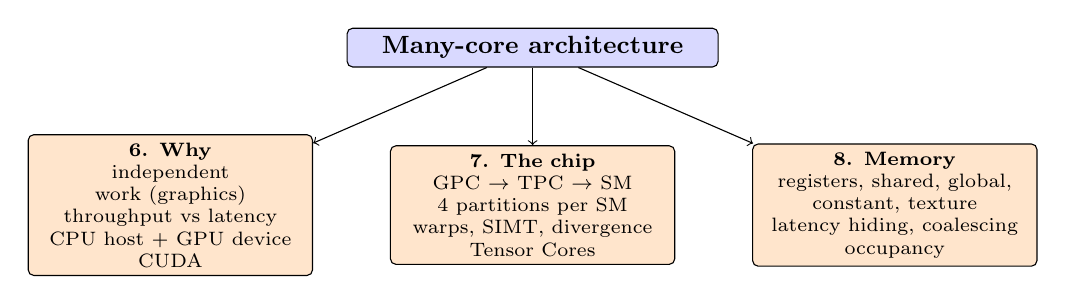
\begin{tikzpicture}[bx/.style={draw,rounded corners=2pt,fill=#1,font=\scriptsize,align=center,inner sep=3pt,text width=3.4cm}]
  \node[bx=blue!15,text width=4.5cm,font=\small\bfseries] (root) at (0,0) {Many-core architecture};
  \node[bx=orange!20] (a) at (-4.6,-2.0) {\textbf{6. Why}\\independent work (graphics)\\throughput vs latency\\CPU host + GPU device\\CUDA};
  \node[bx=orange!20] (b) at (0,-2.0) {\textbf{7. The chip}\\GPC $\to$ TPC $\to$ SM\\4 partitions per SM\\warps, SIMT, divergence\\Tensor Cores};
  \node[bx=orange!20] (c) at (4.6,-2.0) {\textbf{8. Memory}\\registers, shared, global,\\constant, texture\\latency hiding, coalescing\\occupancy};
  \foreach \n in {a,b,c} \draw[->] (root) -- (\n);
\end{tikzpicture}
\end{center}

\begin{keyidea}
A GPU gets its speed from \emph{width}, not from the speed of one thread: thousands of simple units, fed by
a huge number of cheaply-switched threads, with a fast but small on-chip memory that the programmer manages. The cost is that
the program must expose a great deal of regular data parallelism, and must reuse data on chip.
\end{keyidea}

\section{Fact and formula sheet}

\begin{center}
\small
\begin{tabularx}{\linewidth}{@{}l X@{}}
\toprule
\textbf{Topic} & \textbf{Fact}\\
\midrule
Hierarchy & GPU $\supset$ GPCs $\supset$ TPCs $\supset$ SMs ($2$ per TPC) $\supset$ $4$ partitions\\
A100 product & $7$ GPCs, $54$ TPCs, $108$ SMs; full GA100: $8$ GPCs, $64$ TPCs, $128$ SMs\\
Per SM (A100) & $64$ FP32, $64$ INT32, $32$ FP64, $4$ Tensor Cores, $65\,536$ registers ($256$~KB), $192$~KB L1/shared\\
Per chip (A100) & $6912$ FP32 cores, $3456$ FP64, $432$ Tensor Cores, $40$~MB L2, $40$ (or $80$)~GB HBM2\\
Warp & $32$ threads executed in lock-step; one scheduler per partition issues one warp-instruction per clock\\
SM limits (A100) & $2048$ threads ($64$ warps), $32$ blocks, $1024$ threads per block, $255$ registers per thread\\
Peak rate & $\text{units}\times2\times f$ ($2$ for fused multiply-add): FP32 $=6912\times2\times1.41\text{ GHz}=19.5$ TFLOPS\\
Tensor Core rate & $1024$ FMA/clk/SM; $108\times1024\times2\times1.41\text{ GHz}=312$ TFLOPS (FP16, dense)\\
HBM2 bandwidth & $\tfrac{\text{width}}{8}\times\text{clock}\times2=\tfrac{5120}{8}\times1215\text{ MHz}\times2=1555$ GB/s\\
Machine balance & peak FLOP/s $\div$ bandwidth $=19.5/1.555\approx12.5$ FLOP/B\\
Occupancy & resident warps $\div$ $64$; limited by registers: threads $\le65\,536/r$\\
Latencies & global $\approx200$--$400$ cycles; shared $\approx20$--$30$ cycles\\
Little's law & data in flight $=$ bandwidth $\times$ latency\\
Divergence & warp time $=$ sum of the times of the paths taken by its threads\\
Coalescing & consecutive threads $\to$ consecutive addresses: $1$ transaction per $128$~B; stride $\Rightarrow$ up to $32$\\
Bank conflicts & $32$ banks $\times4$~B; conflict if two threads of a warp use different words of one bank\\
Kepler K40 & $15$ SMX $\times192$ SP $=2880$ cores, $65\,536$ registers, $64$~KB shared/L1 (split $16/32/48$)\\
\bottomrule
\end{tabularx}
\end{center}

\section{Self-test questions}

\begin{enumerate}
  \item Why did graphics lead to a design with thousands of weak cores? What is the difference between a latency-oriented and a throughput-oriented chip?
  \item What runs on the host, what on the device, and what are the costs of moving between them?
  \item Draw the hierarchy of the A100 with the numbers at each level, and explain the $64$-versus-$54$ TPC inconsistency on the slides.
  \item Draw one SM and label the four partitions and their contents. Which parts are shared by the partitions?
  \item What is a warp? What is SIMT, and how does it differ from SIMD? What is branch divergence and when does it cost?
  \item What is a Tensor Core? Derive the $312$ TFLOPS figure.
  \item List the CUDA memory spaces with scope and access rights. Where is each physically?
  \item Why can a kernel run out of registers, and what does that do to occupancy?
  \item How does a GPU hide a $300$-cycle memory latency? How many bytes must be in flight to saturate the A100's HBM2?
  \item What is coalescing? What is a bank conflict? Give an access pattern for each.
  \item Name the two differences between GPU threads and CPU threads from slide~15 and what they imply for programming.
\end{enumerate}

\section{How this connects to what comes next}

\begin{itemize}
  \item \textbf{CUDA programming}: grids, blocks and threads are the programmer's names for what Chapters~\ref{ch:a100}--\ref{ch:gpumem} showed in hardware. Block size, shared-memory use and register use decide occupancy.
  \item \textbf{Parallelisation principles}: the idea of exposing enough independent work and reusing data (locality) carries over from CPUs to GPUs.
  \item \textbf{PRAM and parallel algorithms}: the SIMT model with a grid of threads and a shared memory is the nearest real machine to the PRAM model.
\end{itemize}

\section{Glossary}

\begin{description}[leftmargin=2.2cm,labelwidth=2cm,style=nextline,itemsep=2pt]
  \item[Arithmetic intensity] FLOPs performed per byte moved from memory.
  \item[Bank conflict] Two threads of a warp using different words in the same shared-memory bank; the accesses are serialised.
  \item[Branch divergence] Threads of one warp taking different paths at a branch; the paths are executed one after the other.
  \item[Coalescing] Combining the memory accesses of a warp into few transactions.
  \item[CUDA] NVIDIA's architecture, programming model and C-based language for GPUs.
  \item[Device / host] The GPU and its memory / the CPU and its memory.
  \item[FMA] Fused multiply-add, $a\leftarrow a+b\cdot c$; counts as two FLOPs.
  \item[Global memory] Off-chip device DRAM visible to all threads and the host.
  \item[GPC / TPC] Graphics Processing Cluster / Texture Processing Cluster: groups of SMs (a TPC has two).
  \item[HBM2] High-bandwidth memory: stacked DRAM next to the GPU on one package.
  \item[Heterogeneous] Containing different kinds of processors (CPU + GPU).
  \item[Kernel] A function executed on the GPU by many threads.
  \item[Latency hiding] Keeping the units busy with other threads while some threads wait for memory.
  \item[Local memory] Per-thread private memory that physically lives in device DRAM (register spills, big arrays).
  \item[MMA] Matrix multiply-accumulate, $D=AB+C$, the Tensor Core operation.
  \item[Occupancy] Resident warps divided by the maximum number of warps per SM.
  \item[SFU] Special function unit ($\sin$, $\sqrt{\ }$, reciprocal, \dots).
  \item[Shared memory] On-chip scratch-pad shared by the threads of a block.
  \item[SIMT] Single instruction, multiple threads: warp-wise lock-step execution of scalar-style thread code.
  \item[SM / SMX] Streaming multiprocessor (SMX in the Kepler generation).
  \item[SP] Streaming processor: an older name for a GPU core.
  \item[Tensor Core] Matrix-multiply unit of the SM.
  \item[Thread block] Group of threads scheduled together on one SM, sharing shared memory.
  \item[Warp] Group of $32$ threads executed together.
\end{description}

\section{References for further reading}

\begin{itemize}
  \item NVIDIA, \emph{NVIDIA A100 Tensor Core GPU Architecture} whitepaper (2020): the reading recommended in the course; numbers in this part are taken from it.
  \item D.~Kirk, W.-m.~Hwu, \emph{Programming Massively Parallel Processors}: a textbook on GPU architecture and CUDA programming.
  \item NVIDIA, \emph{CUDA C++ Programming Guide}: the authoritative description of the programming model, memory spaces, coalescing and bank rules.
  \item The figures on slides 5--6, 8--9 and 11 are from NVIDIA's whitepapers; slide~12 is from an NVIDIA CUDA course. The diagrams in these notes are original.
\end{itemize}
